%
%	Theorieteil
%

\pagebreak
\section{Data Exploration}

\onehalfspacing

\subsection{Overall Access}

I enabled Plausible web analytics on the blog only six months ago. Let's start with an overall view of people accessing the blog during the last months:

\begin{figure}[H]
\centering
\caption {Overall Access}
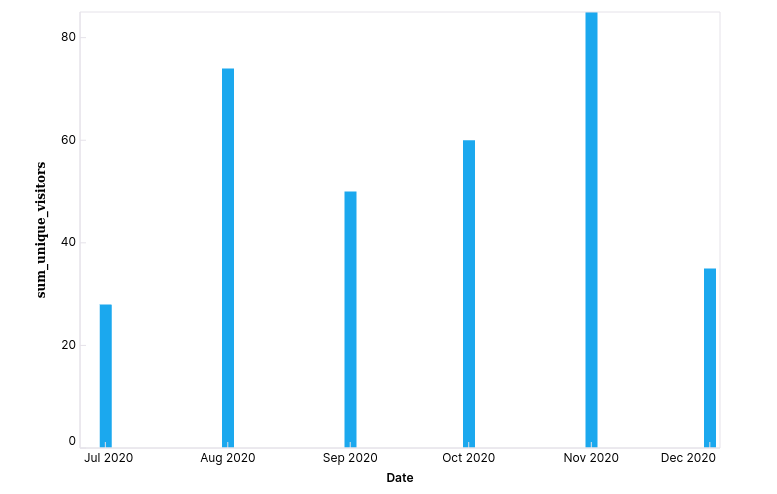
\includegraphics[width=\linewidth]{images/access-overall.png}
\label{fig:accessOverall}
\end{figure}

Looking at the number of unique visitors, we can see a spike in August, most likely in preparation for the latest global climate strike and in November, when the second lockdown started. I would assume that the figures for December are probably a bit too low as I have collected the data before the end of the month.

\subsection{Access by Country}

Where do all the visitors of the blog come from? Let's first have a look at the distribution by country:

\begin{figure}[H]
\centering
\caption {Access by Country}
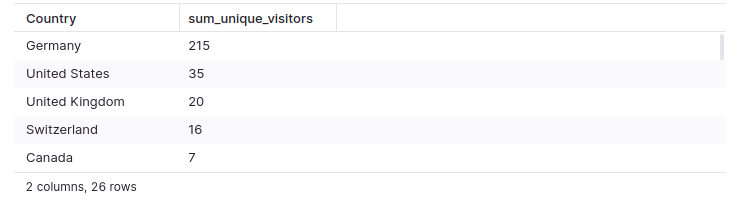
\includegraphics[width=\linewidth]{images/access-country.png}
\label{fig:accessCountry}
\end{figure}

Not surprisingly, most visitors access the blog from Germany, my home country, immediately followed by the United States and the United Kingdom as the blog's language is English. Looking at the access from German-speaking countries, I might get a higher number of visitors if the blog was in German, but I would loose all vistors from countries other than Germany, Austria and Switzerland. For now, I will keep writing blog posts in English.

\subsection{Access by Operating System}

The blog's visitors not only originate from countries, but also from operating systems:

\begin{figure}[H]
\centering
\caption {Access by Operating System}
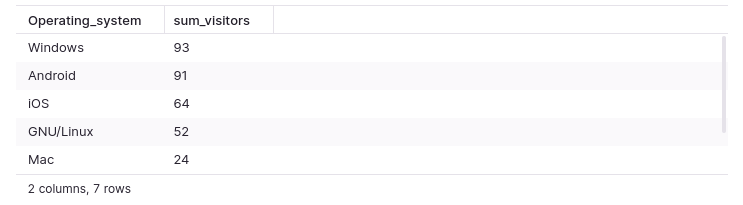
\includegraphics[width=\linewidth]{images/access-os.png}
\label{fig:accessOS}
\end{figure}

and browsers:

\begin{figure}[H]
\centering
\caption {Access by Browser}
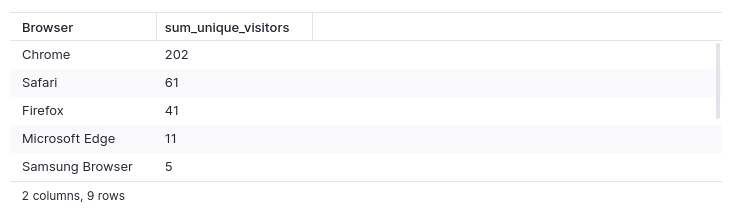
\includegraphics[width=\linewidth]{images/access-browser.png}
\label{fig:accessBrowser}
\end{figure}

Chrome is still the undisputed market leader in browsing and I do know that the WordPress theme in use for the blog displays well on Chrome. 

Looking at the operating system, we can deduct that there is about equal access from mobile devices (Android + iOS) and Desktop devices (Windows + Linux + Mac), so I will need to make sure that the WordPress theme is well suited for mobile devices too.

\subsection{Access by Referral}

In addition to the number of visitors, there are other interesting KPIs, especially visit duration and bounce rate. Let's look at these KPIs first by referral:

\begin{figure}[H]
\centering
\caption {Access by Referral}
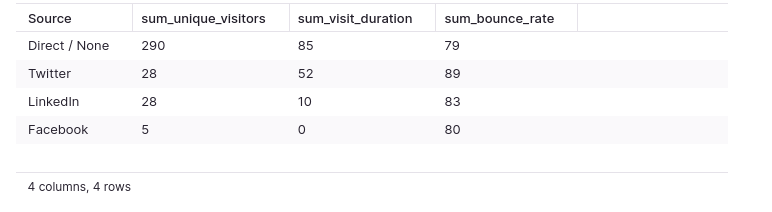
\includegraphics[width=\linewidth]{images/access-referral.png}
\label{fig:accessReferral}
\end{figure}

We can see that direct access to the blog has the most unique visitors, the longest visit duration, and the lowest bounce rate. This is not surprising, people who actively seek out the blog most likely do have the highest interest in its content.

My cross-posts to Twitter, LinkedIn, and Facebook yield a lot fewer visits, with Facebook being the outlier, yielding almost no visitors and no visit duration. In the future I might review cross-posting to Facebook and stop the practice if the numbers do not improve. 

I did not expect the cross-posts to LinkedIn to yield any visits and am pleasantly surprised; without looking at the data I would have assumed that access from Facebook would be much higher than from LinkedIn.

\subsection{Access by Source}

Second, let's look at these KPIs by source:

\begin{figure}[H]
\centering
\caption {Access by Source}
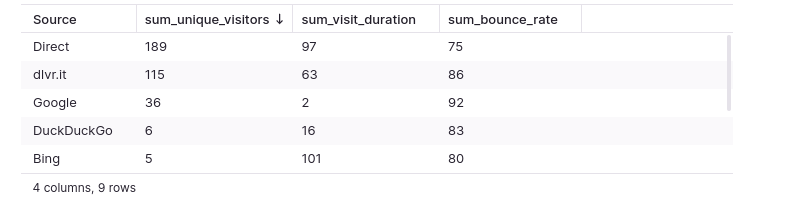
\includegraphics[width=\linewidth]{images/access-source.png}
\label{fig:accessSource}
\end{figure}

As expected we can see the same picture here, direct access to the blog has the highest number of unique visitors, the longest visit duration, and the lowest bounce rate.

Access from the search engines though is a lot less than from cross-posting, which I did not expect. To improve this I might need to review the Google Search Console settings and pay closer attention to tags and keywords.

Only by looking at the data I was already able to gain some insights into the behavior of the visitors of my blog's and identify some possible improvements for the future.

\subsection{Categories}

As a next data point, we'll want to look at the content of the blog posts. First, we'll have a look at the list of categories provided by the blog:

\begin{itemize}
\item buddhism
\item climateaction
\item climateemergency
\item climatestrike
\item cloudnative
\item electric-cars
\item fridaysforfuture
\item kubernetes
\item leavenoonebehind
\item movies
\item music
\item politics
\item rancher
\item socialmedia
\item travel
\item university
\item youtube
\end{itemize}

From the blog's categories I have omitted two, cologne and general, as they are present on all posts. These catgerories are at the same time hashtags for Diaspora*, another social network that I cross-post to; Diaspora* is part of the Fediverse and does not have the same reach as the more popular commercial networks and thus did not appear in the statistics above. Interactions on Diaspora* are far fewer than on the other networks, but they tend to be more thoughtful and more interesting.

To prepare for the analysis I have decided to reduce the number of categories down to four, based on the distribution of the posts in the WordPress dashboard:

\begin{itemize}
\item Climate and politics (1)
\item Cloud (2)
\item Social Media and culture (3)
\item Covid-19 (4)
\end{itemize}

Climate and politics will include all posts regarding the climate emergency and the climate justice movement.

Cloud will include all posts in regards to cloud-native technology.

Social Media and culture will include posts on YouTube, music and movies.

Covid-19 will cover all posts related to the other crisis, the current global pandemic.

 If there's a blog post without category, I will encode the missing value with 0.

These four content categories should help us in the next chapter analyzing the individual blog post performance and possibly arrive at more insights and some predictions.

\subsection{Blog Post Sentiment}

The final data point to explore is the sentiment of the post.

From the many available libraries for Python I've chosen VADER (Valence Aware Dictionary and sEntiment Reasoner) based on the description of the algorithm and its results in an analysis and ranking of texts by H.P. Lovecraft.\footnote{See \textit{Pocs, M. (2018)}: Lovecraft with Natural Language Processing .\cite{lovecraftAnalysis}}.

Vader is "specifically attuned to analyzing social media posts"\footnote{\textit{Hutto, C. (2018)}: VADER Sentiment Analysis .\cite{vaderReadme}} and thus the perfect choice to analyze blog posts; Vader can also be used just with a few lines of code, making it an ideal library for casual analysis. 

With a large data set there would have been the option to create and train a more specific NLP machine learning model to identify the post's sentiment, but for a small data set like the blog I felt it would be more prudent to use a ready-made library.

Let's look at an example invocation:

\begin{lstlisting}[caption=Vader invocation, frame=single, basicstyle=\ttfamily]
from vaderSentiment.vaderSentiment 
  import SentimentIntensityAnalyzer

blogPost = "My first ever entirely virtual Christmas and 
  it went quite well! And so will New Years, I hope."

analyzer = SentimentIntensityAnalyzer()

print(analyzer.polarity_scores(blogPost))
\end{lstlisting}

The text in the example is the first sentence of the most recent post and Vader will show the following sentiment rating:

\verb|{'neu': 0.74, 'compound': 0.68, 'neg': 0.0, 'pos': 0.26}|

From the documentation we know that compound is the normalized, weighted composite score of the other three values (positive, negative and neutral) and the value I'll be using to enrich our data.\footnote{See \textit{Hutto, C. (2018)}: VADER Sentiment Analysis .\cite{vaderReadme}} Compound will have values between 1 (most positive) and -1 (most negative) and there won't be any missing values; a value of 0 will indicate a completely neutral text.

\subsection{Data Source}

For the data analysis and visualization in this chapter I use a Count data notebook, you can find the raw data and all charts from this chapter here: \href{https://count.co/n/6WKuBzDV4Qq}{WTA Chapter 3}
